% 请确保文件编码为utf-8,使用XeLaTex进行编译,或者通过overleaf进行编译

\documentclass[answers]{exam}  % 使用此行带有作答模块
% \documentclass{exam} % 使用此行只显示题目

\usepackage{xeCJK}
\usepackage{zhnumber}
\usepackage{graphicx}
\usepackage{hyperref}
\usepackage{amsmath}
\usepackage{booktabs}
\usepackage{enumerate}
\usepackage{amssymb}
\usepackage{pgfplots} 

\pagestyle{headandfoot}
\firstpageheadrule
\firstpageheader{南京大学}{机器学习导论}{习题一}
\runningheader{南京大学}
{机器学习导论}
{习题一}
\runningheadrule
\firstpagefooter{}{第\thepage\ 页(共\numpages 页)}{}
\runningfooter{}{第\thepage\ 页(共\numpages 页)}{}


\setlength\linefillheight{.5in}

\renewcommand{\solutiontitle}{\noindent\textbf{解:}\par\noindent}

\renewcommand{\thequestion}{\zhnum{question}}
\renewcommand{\questionlabel}{\thequestion .}
\renewcommand{\thepartno}{\arabic{partno}}
\renewcommand{\partlabel}{\thepartno .}


\begin{document}
\Large
\noindent 
% 姓名学号
姓名:杜兴豪 \\
学号:201300096 \\
\begin{questions}
\question [30] \textbf{概率论基础}

	教材附录C介绍了常见的概率分布.
给定随机变量$X$的概率密度函数如下,
\begin{equation}
	f_X(x) = 
	\begin{cases}
		\frac{1}{4} & 0<x<1;\\
		\frac{3}{8} & 3<x<5;\\
		0			& \mbox{otherwise.}
	\end{cases}
\end{equation}

\begin{enumerate}
\item  请计算随机变量$X$的累积分布函数$F_X(x)$;
\item  随机变量$Y$定义为$Y = 1/X$, 求随机变量$Y$对应的概率密度函数$f_Y(y)$;
\item  试证明, 对于非负随机变量$Z$, 如下两种计算期望的公式是等价的.
\begin{equation}
	\label{ch1-eq-expect-1}
	\mathbb{E}[Z] = \int_{z=0}^{\infty}zf(z) \mathrm{d} z.
\end{equation}

\begin{equation}
	\label{ch1-eq-expect-2}
	\mathbb{E}[Z] = \int_{z=0}^{\infty}\Pr[Z\geq z] \mathrm{d} z.
\end{equation}
同时, 请分别利用上述两种期望公式计算随机变量$X$和$Y$的期望, 验证你的结论.
\end{enumerate}
	\begin{solution}
	$
	\begin{aligned}
	&\\1.\\
	&F_X(x)=\int_{-\infty}^x f_X(t)dt=
		\begin{cases}
			0 &x\le0\\
			\frac x4 &0<x<1\\
			\frac 14 &1\le x\le3\\
			\frac{3x-7}8 &3<x<5\\
			1 &O.T.W.\\
		\end{cases}\\\\
	\end{aligned}
  	\\\\2.\\
	\begin{aligned}
	&\because F_Y(y) = P(Y\le y)=P(\frac1X<y)=P(X>\frac1y)=1-P(X\le \frac1y)\\
	&\therefore F_Y(y) = 1-F_X(\frac1y)=
	\begin{cases}
		0 &\frac1y\le0\\
		\frac 1{4y} &0<\frac1y<1\\
		\frac 14 &1\le \frac1y\le3\\
		\frac{3-7y}{8y} &3<\frac1y<5\\
		1 &O.T.W.\\
	\end{cases}\\
	&\therefore F_Y(y)=	\begin{cases}
		0 &y\le0\\
		\frac{3-7y}{8y} &\frac15<y<\frac13\\
		\frac 14 &\frac13\le y\le 1\\
		\frac 1{4y} &y>1\\
		1 &O.T.W.\\
	\end{cases}\\
	&\therefore f_Y(y)=
		\begin{cases}
			-\frac{3}{8y^2}&\frac15<y<\frac13\\
			-\frac1{4y^2}&1\le \frac1y\le3\\
			0&O.T.W.\\
		\end{cases}\\
	\end{aligned}
	\\3.\\
	\begin{aligned}
	&(2)\to E[Z]=\int^{\infty}_0zf(z)dz=\int^{\infty}_0zdF(z)=zF(z)|^{\infty}_0-\int^{\infty}_0F(z)dz\\
	&\because F(\infty) = 1, F(0) = 0\\
	&\therefore E[Z] = z|^{\infty}_0-\int^{\infty}_0F(z)dz=\int^{\infty}_0dz-\int^{\infty}_0F(z)dz\\
	&\therefore E[Z] = \int^{\infty}_0(1-F(z))dz\quad\quad\quad\quad\quad\quad\quad\quad(4)\\
	&(3)\to E[Z]=\int^{\infty}_0\Pr[Z>z]dz=\int^{\infty}_0(1-\Pr[Z<z])dz\\
	&\because F(z)=\Pr[Z<z]\\
	&\therefore E[Z]= \int^{\infty}_0(1-F(z))dz\quad\quad\quad\quad\quad\quad\quad\quad(5)\\
	&(4) = (5)\\
	\end{aligned}
	$
	\end{solution}


\question [40] \textbf{评估方法}

	教材2.2.3节描述了自助法~(bootstrapping), 下面考虑将自助法用于对统计量估计这一场景, 并对自助法做进一步分析. 
考虑$m$个从分布$p(x)$中独立同分布抽取的(互不相等的)观测值$x_1, x_2, \ldots, x_m$, $p(x)$的均值为$\mu$, 方差为$\sigma^2$. 通过$m$个样本, 可使用如下方式估计分布的均值
\begin{equation}
\bar{x}_m = \frac{1}{m} \sum_{i=1}^{m} x_{i}\;,\label{ch2_eq:estimate_mean}
\end{equation}
和方差
\begin{equation}
\bar{\sigma}^2_m=\frac{1}{m-1} \sum_{i=1}^{m}\left(x_{i}-\bar{x}_m\right)^{2}\label{ch2_eq:estimate_variance}
\end{equation}
设$x^*_1, x^*_2, \ldots, x^*_m$为通过自助法采样得到的结果, 且
\begin{equation}
\bar{x}^*_m = \frac{1}{m} \sum_{i=1}^{m} x^*_{i}\;,
\end{equation}
\begin{enumerate}
    \item 请证明$\mathbb E[\bar{x}_m] = \mu$且$\mathbb E[\bar{\sigma}^2_m] = \sigma^2$;
    \item 计算$var[\bar{x}_m]$;
    \item 计算$\mathbb E[\bar{x}^*_m \mid x_1, \ldots, x_m]$和$var[\bar{x}^*_m \mid x_1, \ldots, x_m]$;
    \item 计算$\mathbb E[\bar{x}^*_m]$和$var[\bar{x}^*_m]$;
    \item 针对上述证明分析自助法和交叉验证法的不同.
\end{enumerate}
	\begin{solution}
		$
		\\1.\\
		\begin{aligned}
			&E[\overline x_m]=E[\frac1m\sum^n_{i=1}x_i]=\frac1m\sum^m_{i=1}E[x_i]=\frac1m\sum^m_{i=1}\mu=\mu\\
			&\because Var(\overline x_m)=\frac{\sum^m_{i=1}Var(x_i)}{m^2}=\frac{\sigma^2}m\\
			&\therefore E[\overline x^2_m]=Var(\overline x_m) + E^2[\overline x_m]=\frac{\sigma^2}m+\mu^2\\
			&\therefore E[\sigma^2_m]=\frac1{m-1}\sum^m_{i=1}E[(x_i-\overline x_m)^2]\\		
		\end{aligned}\\
		\begin{aligned}
			&=\frac1{m-1}[\sum^m_{i=1}E[x_i^2]-2E\sum^m_{i=1}x_i\overline x_m+\sum^m_{i=1}E[\overline x_m^2]]\\
			&=\frac1{m-1}[\sum^m_{i=1}E[x_i^2]-2mE[\overline x^2_m]+mE[\overline x_m^2]]\\
			&=\frac1{m-1}[m(\sigma^2+\mu^2)-m(\frac{\sigma^2}m+\mu^2)]=\frac1{m-1}(m-1)\sigma^2=\sigma^2\\	
			\\2.\\
			&\mathsf{Learn\ from\ 1.:}Var(\overline x_m)=\frac{\sigma^2}m\\
		\\3.\\
			&E[\overline x^*_m|x_1,\dots,x_m]=\frac1m\sum^m_{i=1}E[x^*_i|x_1,\cdots,x_m]=\frac{\sum\limits^m_{i=1}x_i}m=\overline x_m\\
			&Var[\overline x^*_m|x_1,\dots,x_m]=\frac1{m-1}\sum^m_{i=1}(x_i^*-E[\overline x^*_m|x_1,\dots,x_m])^2=\overline \sigma^2_m\\
		\\4.\\
			&E[\overline x^*_m]=\frac1m\sum^m_{i=1}E[x^*_i]=\frac1m\sum^m_{i=1}\mu=\mu\\
			&Var[x^*_i]=Var(x)=\sigma^2\\
			&Var[\overline x^*_m]=\frac1{m^2}Var[\sum^m_{i=1}x^*_i]=\frac{\sum^m_{i=1}Var(x^*_i)}{m^2}=\frac{\sigma^2}m\\
		\\5.\\
		\end{aligned}\\
		$
		自助法是基于样本总体进行多次有放回抽样的新数据集进行学习,而交叉验证法则通过严格区分训练集和测试集的方式,多次划分取平均值来进行学习。\\
		在以p(x)的分布作为数据集进行学习时,交叉验证法的某一次划分中,得到的结果可能是具有较大误差的,然而在进行平均值计算后可以得到一个比较好的水平;而在自助法中,我们计算的模型是通过自助取样得到的,与初始数据集的分布有一定的偏差,导致我们计算结果即使再精确,也有可能难以达到预期的效果。\\
		但是在第三问中,以x1到xm这个比较小的数据集进行学习时,可以看出计算结果和其真正均值和方差相同,自助法可以发挥出比较好的水平。
	\end{solution}


\question [30] \textbf{性能度量}

	教材2.3节介绍了机器学习中常用的性能度量. 假设数据集包含8个样例, 其对应的真实标记和学习器的输出值(从大到小排列)如表~\ref{table:roc}所示. 该任务是一个二分类任务, 标记1和0表示真实标记为正例或负例.
学习器的输出值代表学习器认为该样例是正例的概率. 
\begin{table}[!h]
	\centering
	\caption{样例表} \vspace{2mm}\label{table:roc}
	\begin{tabular}{c|c c c c c c c c c c c}\toprule
		样例 & $x_1$ & $x_2$ & $x_3$  & $x_4$  & $x_5$& $x_{6}$& $x_{7}$ & $x_{8}$  \\
		\midrule
		标记 & 1  & 1 &  0 &  1  & 0 & 1 & 0 & 0\\
		\midrule
		分类器输出值 & 0.81 &  0.74 &  0.62  & 0.55 & 0.44 &0.35 & 0.25 & 0.21\\
		\bottomrule
	\end{tabular}
\end{table}
\begin{enumerate}
    \item 计算P-R曲线每一个端点的坐标并绘图;
    \item 计算ROC曲线每一个端点的坐标并绘图, 计算AUC;
\end{enumerate}
	\begin{solution}
		$
	    \begin{aligned}
			&\quad\quad P=\frac{TP}{TP+FP},\quad\quad R=\frac{TP}{TP+FN}\\
			\therefore&P_1=\frac{1}{1+0}=1,&&R_1=\frac{1}{1+3}=\frac14=0.25\\
			&P_2=\frac{2}{2+0}=1,&&R_2=\frac{2}{2+2}=\frac12=0.5\\
			&P_3=\frac{2}{2+1}=\frac23=0.67,&&R_3=\frac{2}{2+2}=\frac12=0.5\\
			&P_4=\frac{3}{3+1}=\frac34=0.75,&&R_4=\frac{3}{3+1}=\frac34=0.75\\
		\end{aligned}\\
		\begin{aligned}
			&P_5=\frac{3}{3+2}=\frac35=0.6,&&R_5=\frac{3}{3+1}=\frac34=0.75\\
			&P_6=\frac{4}{4+2}=\frac23=0.67,&&R_6=\frac{4}{4}=1\\
			&P_7=\frac{4}{4+3}=\frac47=0.57,&&R_7=\frac{4}{4}=1\\
			&R_8=\frac{4}{4+4}=\frac12=0.5,&&R_8=\frac{4}{4}=1\\
		\end{aligned}\\
		$
		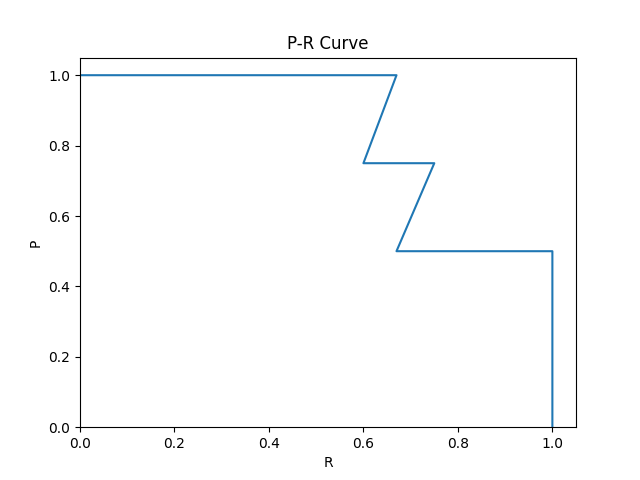
\includegraphics{Figure_1.png}
		$
		\begin{aligned}
			&\quad\quad TPR=\frac{TP}{TP+FN}\quad\quad FPR=\frac{FP}{TN+FP}\\
			\therefore&TPR_1=\frac{1}{4}=0.25,&&FPR_1=\frac{0}{4}=0\\
			&TPR_2=\frac{2}{4}=0.5,&&FPR_2=\frac{0}{4}=0\\
			&TPR_3=\frac{2}{4}=0.5,&&FPR_3=\frac{1}{4}=0.25\\
			&TPR_4=\frac{3}{4}=0.75,&&FPR_4=\frac{1}{4}=0.25\\
			&TPR_5=\frac{3}{4}=0.75,&&FPR_5=\frac{2}{4}=0.5\\
			&TPR_6=\frac{4}{4}=1,&&FPR_6={2}{4}=0.5\\
			&TPR_7=\frac{4}{4}=1,&&FPR_7=\frac{3}{4}=0.75\\
			&TPR_8=\frac{4}{4}=1,&&FPR_8=\frac44=1\\
		\end{aligned} \\
		$
		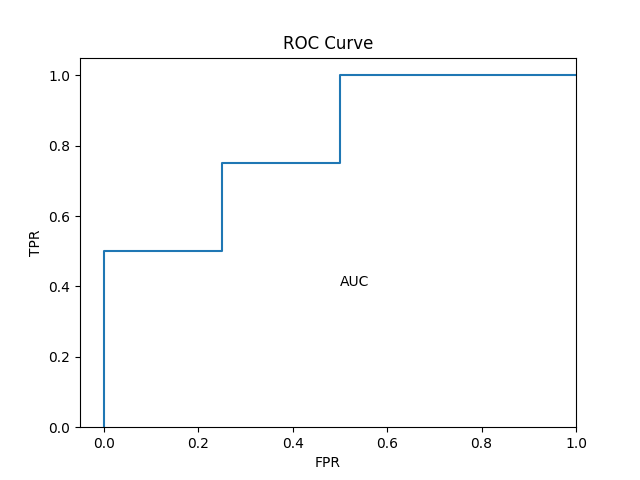
\includegraphics{Figure_2.png}
		$
		AUC = 0.5\times 0.25+0.75\times0.25+1\times0.5=0.8125
		$
	\end{solution}
\end{questions}
\end{document}